\documentclass[12pt, english]{report}
\usepackage{subcaption}
\usepackage{amsmath}
\usepackage{amssymb}
\usepackage{stackrel}
\usepackage{graphicx}
\usepackage{hyperref}
\usepackage{caption}
\usepackage[noadjust]{cite}
\usepackage{authblk}
\usepackage{placeins}
\usepackage{adjustbox}
\usepackage{tabularx}
\usepackage{graphics}
\usepackage[nottoc]{tocbibind}
\usepackage{ragged2e}
\usepackage{etoolbox}
\usepackage{subcaption}
\usepackage{float}
\usepackage{babel}
\usepackage[a4paper, total={6in, 10in}]{geometry}
\usepackage{booktabs}
\usepackage{colortbl}
\usepackage{xcolor}
\usepackage{xfrac}
\usepackage{listings}
\usepackage{color} %red, green, blue, yellow, cyan, magenta, black, white
\definecolor{mygreen}{RGB}{28,172,0} % color values Red, Green, Blue
\definecolor{mylilas}{RGB}{170,55,241}


\lstset{language=Matlab,%
    %basicstyle=\color{red},
    breaklines=true,%
    morekeywords={matlab2tikz},
    keywordstyle=\color{blue},%
    morekeywords=[2]{1}, keywordstyle=[2]{\color{black}},
    identifierstyle=\color{black},%
    stringstyle=\color{mylilas},
    commentstyle=\color{mygreen},%
    showstringspaces=false,%without this there will be a symbol in the places where there is a space
    numbers=left,%
    numberstyle={\tiny \color{black}},% size of the numbers
    numbersep=9pt, % this defines how far the numbers are from the text
    emph=[1]{for,end,break},emphstyle=[1]\color{red}, %some words to emphasise
    %emph=[2]{word1,word2}, emphstyle=[2]{style},
}



%%%%%%%%%%%%%%%%%%%%%%%%%%%%%%%%%%%%%%%%%%% for fonts of Abstract  %%%%%%%%%%%%%%%%%%%%%%%%%%%%%%%%%%%%%%%

\usepackage{abstract}
\renewcommand{\abstractnamefont}{\huge\bfseries}


%%%%%%%%%%%%%%%%%%%%%%%%%%%%%%%%%%%%%%%%%%%%%   Adding Biblography/lof/lit in table of content  %%%%%%%%%%%%%%%%%%%%%%%%%%%%%%%%%%%%%%%%%%%%%%%
%\usepackage{tocbibind}

\makeatletter

\begin{document}


\begin{titlepage}
\begin{center}



\includegraphics[width=0.35\textwidth]{./logo}~\\[1.5cm]

%%%%%%%%%%%%%%%%%%%%%%%%%%%%%%%%%%%%%%%%%%%%%%%%%%%%%%%%%%%%%%%%%%%% Title  %%%%%%%%%%%%%%%%%%%%%%%%%%%%%%%%%%%%%%%%%%%%%%%%%%%%%%%%%%%%%%%%%%%%

{ \huge \bfseries Speech Processing Using MATLAB} \\[1.4cm]

{ \large \bfseries Submitted by:} \\[0.2cm]
{ \large \bfseries Hamza Umar}  \\[0.1cm]
{ \small FA19-BCE-026} \\[0.2cm]
{ \large \bfseries Rahim Ullah Khan}  \\[0.1cm]
{ \small FA19-BCE-009} \\[0.2cm]
{ \large \bfseries Muhammad Kaleem Ullah}  \\[0.1cm]
{ \small FA19-BCE-007} \\[0.2cm]
%{ \small \bfseries Usman} \\[0.2cm]
%{ \small \bfseries Kashif} \\[0.2cm]



{ \small \bfseries Program: BS in Computer Engineering} \\[0.2cm]
%{ \small \bfseries Enrollment Number: 1234} \\[1.0cm]


{ \large \bfseries Submitted to:} \\[0.1cm]
{ \small \bfseries  Engr. M Abdul Rehman} \\[1.0cm]


%{ \large \bfseries Co-Supervised by:} \\[0.1cm]
%{ \small \bfseries Engr. Laraib Malik} \\[0.8cm]
%{ \large \bfseries Assistant Professor} \\[0.9cm]
%{ \large \bfseries Department of Electrical Engineering} \\[0.3cm]

\vfill

\textsc{A Project submitted in partial fulfillment of the requirements for the degree of bachelors of Science in Computer Engineering}\\[1cm]


{ \large \bfseries Department of Electrical and Computer Engineering} \\[0.2cm]
{ \large \bfseries COMSATS University Islamabad, Attock Campus, Pakistan.} \\[0.2cm]


% Bottom of the page
%{\large \today}   % Date

\thispagestyle{empty}
\end{center}
\end{titlepage}

% Thesis Dedication ---------------------------------------------------

%\begin{declaration} %this creates the heading for the dedication page
%\chapter*{Declaration}
%\begin{titlepage}

%\noindent {\Large \textbf{Declaration}} \\

%\vspace*{7cm}
\begin{titlepage}
\begin{center}
\noindent {\Large \textbf{Declaration}} \\
\end{center}
  \vspace*{0.5cm}

I declare that the project report SPEECH PROCESSING USING MATLAB is based on our own work carried out during the course of our study under the supervision of Engr. M Abdul Rehman.\\
I assert the statements made and conclusions drawn are an
outcome of my research work. I further certify that\\[0.2cm]

\begin{enumerate}
\item  The work contained in the report is original and has been
done by us under the general supervision of my
supervisor.

\item The work has not been submitted to any other Institution
for any other degree/diploma/certificate in this university
or any other University of Pakistan or abroad.


\item We have followed the guidelines provided by the
university in writing the report.

\item Whenever we have used materials (data, theoretical
analysis, and text) from other sources, we have given due
credit to them in the text of the report and giving their
details in the references.

\end{enumerate}


\end{titlepage}
%\end{declaration}

% ----------------------------------------------------------------------

%\input{PrePages/CertificateofApproval}
%\input{PrePages/PlagiarismUnderTaking}
%\input{PrePages/ListOfPublications}
% Thesis Dedication ---------------------------------------------------

%\begin{dedication} %this creates the heading for the dedication page
%\chapter*{Dedication}
%\begin{titlepage}

%\noindent {\Large \textbf{Dedication}} \\

%\vspace*{7cm}
\begin{titlepage}
\begin{center}
\noindent {\Large \textbf{Dedication}} \\
\end{center}
  \vspace*{0.5cm}

First and foremost we offer our sincerest gratitude to our course instructor,  Engr. M Abdul Rehman, Who encouragement, guidance and support from the initial to the final level enabled us to develop an understanding of the subject. Without his guidance and persistent help this project would not have been possible.\\[0.2cm]
To our parents, we would like to thank to them for supporting us in our daily lives, for going to school every day, and having them by our side to guide us always, their prosperity and love for us.
\end{titlepage}
%\end{dedication}

% ----------------------------------------------------------------------

%%% Local Variables:
%%% mode: latex
%%% TeX-master: "../thesis"
%%% End:

\begin{titlepage}
\begin{center}
\noindent {\Large \textbf{Acknowledgements}} \\
\end{center}
  \vspace*{0.5cm}
\noindent Thanks to ALLAH (s.w.t), the Greatest, the most Merciful and the most Gracious, Whose countless blessings bestowed upon me kind, talented and wise teachers, who provided me sufficient opportunities, and enlighten me towards this research work.\vspace{.25cm}

\noindent I would like to extend my deepest thanks to our project supervisor, Engr. M Abdul Rehman for giving ua the opportunity of undertaking this project under his determined directions. His support, dedication, encouragement, excellent supervision and guidance are what made this thesis possible. \vspace{.25cm}

\noindent Thanks to my beloved family, whose prayers, dedication, support and love are the most precious assets, I had (and I have), during the course of my Engineering work and for all of my endeavors.\vspace{.25cm}

\noindent I am very thankful to the administration and faculty of COMSATS University Islamabad, Attock Campus for providing me a great environment that helped me a lot in conducting our project related activities. \vspace{5mm} \\


\noindent Thank You!

%I am also extremely thankful to Dr. Waseem Ikram, Dr. Aftab Maroof, Dr. Arshad A. Shahid, Dr. Anwar M. Mirza, Dr. Farrukh A. Khan, Dr. Hammad Majeed and Dr. Waseem Shahzad for supporting me in my research work at NUCES.  How can I forget my colleagues (@ FAST): Muhammad Sharif, Mohsin Bilal, Asif Khan, Muhammad Ishtiaq, Hamid, Sajid, Javed, Ahmad, Hameed, Imran, Raees, Israrullah, Israr and all other PhD fellows for their support: intellectually as well as for the stuff, related to enjoyment!\vspace{.25cm}

%\noindent I am extremely thankful to my wife for helping me out in difficult situations. Also, thank you my sister for your love and for cooking the delicious foods that helped me in cooking the recipes of my ideas.\vspace{.25cm}

%\noindent And of course, even if I don't mention, they will get it: a big thank you to my friends: Javed Akhter, M. Nadeem Shahid, Arshad, Rana Khalil, Imran Niazi and M. Imran (hey, order doesn't matter) for offering outdoor enjoyment stuff that is difficult to be mentioned in this tiny document.\vspace{.25cm}

%\noindent Finally, I would like to gratefully acknowledge the financial support received from the Higher Education Commission of Pakistan during the course of my PhD (for almost everything).


\end{titlepage}


\begin{abstract}
Speech processing using MATLAB gives the reader a comprehensive overview of contemporary speech and audio processing techniques with an emphasis on practical implementations and illustrations using MATLAB code.
Speech process refers to the analysis of speech signals and their processing to obtain useful information. Speech processing can also be referred as digital signal processing, as the speech signals are digitized for processing.
Core concepts are first covered in an introduction to the physics of audio and vibration together with their representations using complex numbers,Z transforms, and frequency analysis transforms such as the FFT.\\

Speech processing involves identifying the isolated word from the corresponding
speech signal. From the speech signal that corresponds to the particular word, one or
more features such as linear predictive coefficients (LPC), Mel-frequency cepstral
coefficients (MFCC) (refer Chap.3) are collected and are arranged as the elements to
form the vector. This is known as the feature extraction, and the corresponding vector
is known as feature vector. Every element in the vector is known as the attributes.
Suppose we need to design the digit classifier that classifies the word zero to nine
(digits) from the corresponding speech signal. About large number (several hundreds)
of feature vectors corresponding to the individual digits are collected from the various
speakers to design the speaker-independent classifier. Fifty percent of the collected
data are used for designing the classifier.\\

Speech processing is a computerized speech text process in voice is usually recorded with acoustic microphones by capturing air pressure changes. This kind of air transmitted voice signals is prone to two kinds of problems related to voice robustness and applicability. The former means mixing of speech signals and ambient noise usually deteriorate automatic voice recognition system performance. The latter means speech could be overheard easily on air transmission channel and this often results in privacy loss or annoyance to other people.\\

The following module describes the process behind implementing signal processing techniques in MATLAB. The algorithm utilizes the Discrete Fourier Transform in order to compare the frequency spectra of two voices. Further more, we are comparing and analysing original signal with Fourier Transform to find highest frequency of signal, and decimating re-sampling data at a lower rate after low pass filtering.\\



\vspace{0.89mm}
%\pagenumbering{roman}% added the roman page number in the starting pages
\thispagestyle{empty}% to remove the page number
\end{abstract}

%\input{PrePages/emptypage}
%\input{PrePages/Examiners}
%\input{PrePages/Certificate}

\pagenumbering{roman}
\setcounter{page}{11}


\tableofcontents{}
\pagebreak{}
\listoffigures{}
\pagebreak{}
%\listoftables{}
\pagebreak{}
%\input{PrePages/nomenclature}
%\newpage{}
%\input{PrePages/ListofAbbreviations}


\pagenumbering{roman}
\setcounter{page}{23}

\newpage{}
\pagenumbering{arabic}

%%%%%%%%%%%%%%%%%%%%%%%%%%%%%%%%%%%%%  Chapters  %%%%%%%%%%%%%%%%%%%%%%%%%%%%%%%%%%%%%%%%%%%%%%%%%%%%%%%%%%%%%%%%%

\chapter{Introduction}
\label{chap1}
Signals are time-varying quantities which carry information. They may be, for example, audio signals (speech, music), images or video signals, sonar signals or ultrasound, biological signals such as the electrical pulses from the heart, communications signals, or many other types. With the emergence of high-speed, low-cost computing hardware, we now have the opportunity to analyze and process signals via computer algorithms.\\

The basic idea is straightforward: Rather than design complex circuits to process signals, the signal is first converted into a sequence of numbers and processed via software. By its very nature, software is more easily extensible and more versatile as compared with hard-wired circuits, which are difficult to change. Furthermore, using software, we can build in more �intelligence� into the operation of our designs and thus develop more human-usable devices.
\section{Objectives}
%
%
The objectives of this project are:
%
%for 1,2,3 numbers
\begin{enumerate}
\item To get familiar with how to describe signals mathematically and understand how to perform mathematical
operations on signals.
%
\item It will provide knowledge of digital filter
%
\item To discuss word length issues ,multi rate signal processing and application.
%
%
\end{enumerate}
\section{Introduction}
\noindent Audio signal processing is the subfield of signal processing in which we work with the
audio or what we hear. Different objects produce sound like bird, engines, motors noise
in robotic systems. The human can hear these sounds but there is always a mixture of
some background noise in the audio signals that must be processed in order to
get the desire signals.
\begin{figure}[H]  %h=positioning
\begin{center}
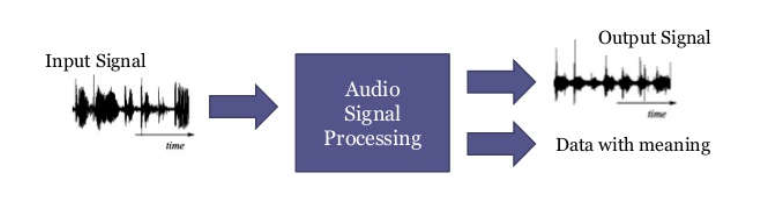
\includegraphics[scale=0.60]{Chapter1/figure1}
\caption{Audio Signal Processing}
\label{figure1}
\end{center}
\end{figure}

The audio sample is taken having some background noise or by adding noise by yourself,
then this audio sample is processed by analyzing it in MATLAB or any other tools. We
perform some operation of the signal, for more precisely analyzing the signals in
Frequency spectrum for analyzing in frequency domain in order to remove noise. Then a
filtered signal is produced at the output.
\begin{figure}[H]  %h=positioning
\begin{center}
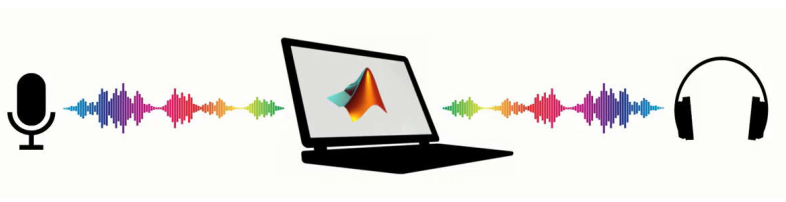
\includegraphics[scale=0.60]{Chapter1/figure2}
\caption{Signal Processing Technique}
\label{figure2}
\end{center}
\end{figure}

\subsection{Filters}
\subsubsection{Bandpass Filters}
A bandpass filter is an filter that allows signals between two explicit frequencies,
however that oppresses signals at different frequencies. Some bandpass channels
require an outer wellspring of intensity and utilize dynamic parts, for example,
semiconductors and coordinated circuits; these are known as dynamic bandpass filters.

\begin{figure}[H]  %h=positioning
\begin{center}
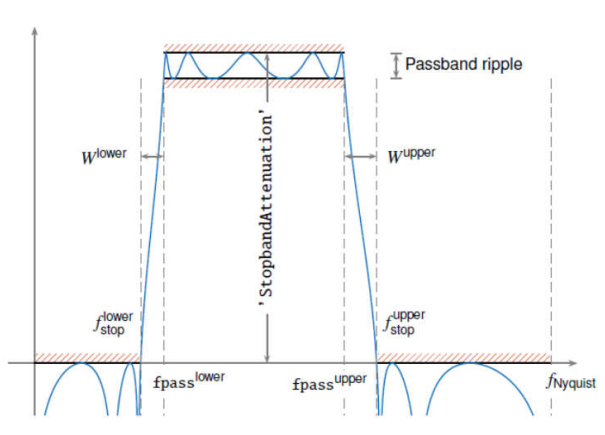
\includegraphics[scale=0.60]{Chapter1/bandPassFilter}
\caption{Band Pass Filter Frequency Response}
\label{bandPassFilter}
\end{center}
\end{figure}

\subsubsection{Band Stop Filters}
The Band Stop Filter, (BSF) is another variety of frequency selective circuit that
functions in just the other thanks to the Band Pass Filter we tend to checked out before.
The band stop filter, additionally referred to as a band reject filter, passes all
frequencies with the exception of these inside a such stop band that are greatly
attenuated.\\
Also, a bit like the band pass filter, the band filter may be a second-order (two-pole)
filter having 2 cut-off frequencies, normally referred to as the -3dB or half-power
points manufacturing a good stop band information measure between these 2 -3dB
points.\\
So for a wide-band band stop filter, the filters actual stop band lies between its lower
and higher -3dB points because it attenuates, or rejects any frequency between
these 2 cut-off frequencies. The frequency response curve of a perfect band stop filter
is so given as:
\begin{figure}[H]  %h=positioning
\begin{center}
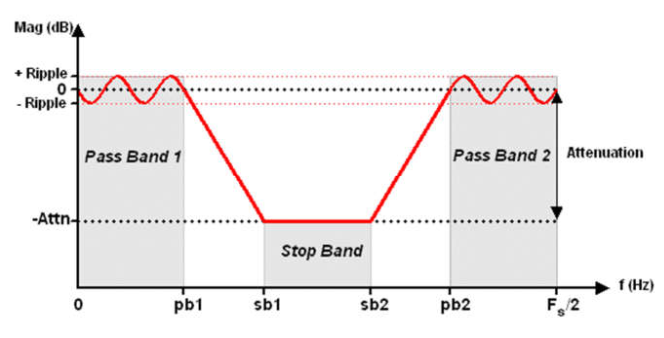
\includegraphics[scale=0.55]{Chapter1/stopBandFilter}
\caption{Band Stop Filter Frequency Response}
\label{stopBandFilter}
\end{center}
\end{figure}

\subsubsection{Low pass Filter}
A low-pass filter is a filter that permits signals under a cutoff frequency (known as the
pass band) and lessens signals over the cutoff frequency (known as the stop band). By
evacuating a few frequencies, the channel makes a smoothing impact. That is, the
channel delivers moderate changes in yield esteems to make it simpler to see patterns
and lift the general SNR with insignificant signal noise.

\begin{figure}[H]  %h=positioning
\begin{center}
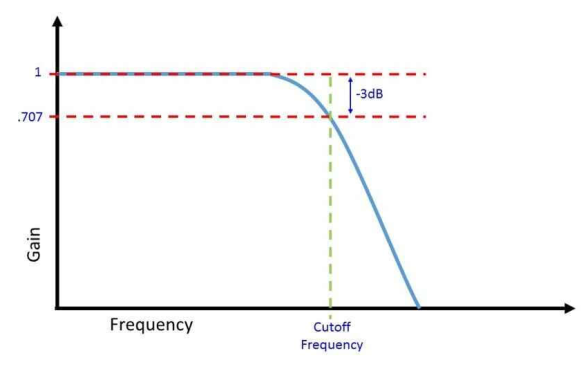
\includegraphics[scale=0.55]{Chapter1/lowPassFilter}
\caption{Low Pass Filter Frequency Response}
\label{lowPassFilter}
\end{center}
\end{figure}

%\section{Motivation}
%Motivated by the emergence of technological advancements and challenges in ...


%
%

%
%\section{UN Stainability Goals}

 %Goal 8 is shown which is Promote sustained, inclusive and sustainable economic growth, full and productive employment and decent work for all. As we will also discuss the economical long time benefits in next chapters. Our project will help industry in economic growth as well as it is providing a help to the meter readers.



%The conceptual frame work for the proposed method is comprises of three basic building blocks and detailed model is shown in Fig. \ref{fw}.
%\begin{enumerate}
%\item Network Formation Block.
%\item Neighbourhood Based Network Matrix Formation Block.
%\item Consensus Formation Block.
%\end{enumerate}
%
%In the network formation block, ...
%
%\FloatBarrier
%\begin{figure}[H]
%\begin{center}
%\hspace{15mm}
%\includegraphics[scale=0.35]{Chapter1/robocanesinternalstates}
%
%\protect\caption{Pseudo-code of Proposed Scheme for Cooperative Control of Networked Multi-Agent Systems.}
%\label{scode}
%\end{center}
%\end{figure}
%
%
\section{Report Break Down}
%
%This thesis deals with convergence analysis .... The main contributions of this work are summarized as follows:
%
%\begin{enumerate}
%\item  Initially a design ....
%
%\item An extended ....
%
%
%\item Modeled a ....
%
%\end{enumerate}
%
%The main contribution of this work is to propose a new way ....
%
%
%
%
%\section{Thesis Outline}
%
%
The major focus of this report is on the findings of the proposed project i.e. Speech Processing Using MATLAB

This Report is organized as follows:
\vspace{5mm}

In chapter 2, literature review is provided in detail about the work which is already been done on speech processing using MATLAB and will give a brief details about the articles, papers and literature review.
\vspace{5mm}


In Chapter 3, Proposed Methodology is presented in which you will be able to see the method we will work on the designing of a complete project source code to the diagrams.

\vspace{5mm}


In Chapter 4, Result and Simulations are being discussed, in which you will see all kind of finding related to the speech processing using MATLAB.


\vspace{5mm}

In Chapter 5, we have concluded and summarized the project work and also presented few new research ideas for future studies.


%\begin{equation}
%F=\sum_{n=0}^i(x_i(0)-x_j(0))^2
%%stackrel[u]{v}{T}=\stackrel[u]{v}{L}+\stackrel[u]{v}{L}\underset{W\epsilon V\cap w\neq u}{\sum}\stackrel[v]{w}{L}
%\end{equation}

\chapter{Literature Review}
\label{chap2}

In the chapter 1 we have given the introduction of our project, objectives and a thesis break down. Our introduction chapter is giving a complete overview of this project report. This chapter is about the work which is already been done on speech processing using MATLAB and will give a brief details about the articles, papers and literature review.

\section{Literature Review}
This chapter is about studies and literatures that are related to the Automatic Meter Reading that the proponents made use of different reading materials (such as thesis, articles, and other web articles) that will help extending the knowledge of the topic. These reading materials will also guide the proponent to improve and develop their proposed system more effectively.

Speech is one of the most important medium by which a communication can take place. With the invention and widespread use of mobiles, telephones, data storage devices etc. has provided a major help in setting up of speech communication and its analysing. The term and the basic concept of speech identification was began in the early 1960`s with exploration into voiceprint analysis which was somewhat similar to fingerprint concept. It was in 1984 that a science fiction called �Star Trek to George Orwell`s,� derived the concept that a machine can recognize the human voice.\cite{mandalia2011speaker}\\
Nowadays, with further growth \& advancement in the field of speech recognition, the humans who are physically challenged such as blind and deaf can easily communicate with the machines. So in biological terms a voice that is being generated through trachea will be decoded by brain.\cite{saxena2013speech}\\

The critical need for computationally efficient and user-friendly numerical software is hardly a matter of any controversy, although a number of key questions still remain wide open. In the current computing hardware landscape, any substantial gains in computational efficiency beyond the well-established best-practice techniques and standard software development tools (compilers, libraries, frameworks, etc.) usually come at the price of an increased customization for the target hardware. Such customizations tend to reduce the portability, readability, and maintainability of the code and frequently require specialized software development tools and skills to use them. The efforts to bridge the chasm between the readability/maintainability of numerical solver packages and the optimum performance on a given hardware are very active right now \cite{lawrence2018crossing} and generally aim to create higher abstraction levels for numerical software development such as domain specific languages (DSLs) paired with code generation capabilities.\cite{kuckuk2018whole},\cite{schulthess2015programming}




%\begin{table}[H]
%%\large
%\centering
%\caption{Consolidated Comparison of all the Systems}
%\label{tab2}
%%begin{adjustwidth}{-2.25in}{Oin}
%
%\begin{tabular}{|c|c|c|c|c|c|}
%\hline  %make a line
%Technology Used&Cost&Feasibility&Reliability&Communication Protocol\\
%\hline %make a line
%GSM&Low&Most Feasible&High&Stable\\
%\hline
%ZigBee&Medium&Small Scale&Low&Least Stable\\
%\hline
%SCADA&High&Not Feasible&High&Stable\\
%\hline
%PLC&Low&Least Feasible&Low&Very Stable\\
%\hline
%WiMAX&Medium&Small Scale&Medium&Stable\\
%\hline
%Mixed&Varies&Feasible&Varies&Varies\\
%\hline
%\end{tabular}
%\end{table}
%
%\small
%\begin{table}[H]
%\caption{Literature Review}
%\label{tab3}
%\centering
%\begin{tabularx}{1\linewidth}{X X X X}
%\toprule
% Paper Reference & Approach & Technology & Accuracy ($\%$) \\
%\toprule
%\cite{khan2020cost}&Cost Benefit Based Analytical Study of AMR and Blind Meter Reading (BMR) used by PESCO(WAPDA)& AMR and BMR &The Blind Meter Reading has internal financial return of about 84 percent while in case of AMR it is 15 percent.\\
%%\toprule
%\hline  %make a line
%\cite{zhao2005research} & Remote Meter Automatic Reading
%Based on Computer Vision & Computer vision techniques & $78\%$\\
%\hline %make a line
%\cite{li2019light} & Light-Weight Spliced Convolution Network-Based
%Automatic Water Meter Reading in Smart City & Network-Based
%Automatic Water Meter Reading & $85.66\%$ \\
%%\toprule
%\hline  %make a line
%\cite{dong2010design} & Wireless AMR System Based on SOPC & SOPC & $59.6\%$ \\
%\hline  %make a line
%\cite{ando2002automatic} & AMR system adopting automatic routing technology & routing technology & $68\%$ \\
%\hline  %make a line
%\cite{wiratama2018gas} & Gas
%billing system based on AMR on diaphragm gas meter with email
%notification & GSM or
%GPRS networks & $79\%$\\
%\hline  %make a line
%\cite{ashna2013gsm} & GSM based automatic AMR system with instant billing & GSM & $88\%$\\
%\hline  %make a line
%\cite{shuo2019digital} & Digital recognition of electric meter with deep learning & Deep Learning Methods & $78\%$\\
%\hline  %make a line
%\end{tabularx}
%\end{table}
%\small
%\begin{table}[H]
%\caption{-- continued from previous Literature Review table \ref{tab3}}
%\label{tab4}
%\centering
%\begin{tabularx}{1\linewidth}{X X X X}
%\toprule
% Paper Reference & Approach & Technology & Accuracy ($\%$) \\
%\toprule
%
%\cite{kulkarni2012gsm} &GSM based AMR system using ARM controller & ARM Controller & $81\%$\\
%\hline  %make a line
%\cite{Ali2012} & Implementation of (AMR) using radio frequency (RF) module & Radio Frequency & $58\%$\\
%\hline  %make a line
%\cite{palaniappan2015automated} & Comparison between different technologies being used in ARM  & GSM, Zigbee, SCADA System, Power Line Communication, WiMAX Technology,  & GSM = $88\%$, Zigbee = $67\%$,SCADA = $63\%$,Power Line = $71\%$,WiMAX = $62\%$,  \\
%\hline %make a line
%\cite{quan2010design} & Design of remote automatic meter reading system based on ZigBee and GPRS & ZigBee and GPRS techniques & $67\%$\\
%\hline  %make a line
%\cite{arun2012design} & Design and implementation of AMR system using GSM, ZIGBEE through GPRS & using GSM, ZIGBEE through GPRS & $89\%$\\
%\hline  %make a line
%\cite{rouf2012neighborhood} & Security and privacy analysis of automatic meter reading systems & Analysises of AMR & -\\
%\hline  %make a line
%\cite{malhotra2013automatic} & AMR and theft control system by using GSM & GSM & $84\%$\\
%\hline  %make a line
%\cite{tan2007automatic} & Automatic power meter reading system using GSM network & GSM network  & $78\%$\\
%\hline  %make a line
%\cite{Jamil2008} & Design and implementation of a wireless AMR system & GSM Network & $86\%$\\
%\hline  %make a line
%\cite{yuan2011remote} & Remote wireless AMR system based on GPRS & GPRS & $88\%$\\
%\hline  %make a line
%\cite{borle2013automatic} & AMR for electricity using power line communication & power line communication & $65\%$\\
%\hline  %make a line
%\end{tabularx}
%\end{table}
%\small
%\begin{table}[H]
%\caption{-- continued from previous Literature Review table \ref{tab4}}
%\label{tab5}
%\centering
%\begin{tabularx}{1\linewidth}{X X X X}
%\toprule
% Paper Reference & Approach & Technology & Accuracy ($\%$) \\
%\toprule
%\cite{mlakic2017designing} & Designing AMR system using open source hardware and software &open source hardware and software & $59\%$\\
%\hline  %make a line
%\cite{khalifa2010survey} & A survey of communication protocols for auto-
%matic meter reading applications, & Communication Protocols & - \\
%\hline
%\bottomrule
%\end{tabularx}
%\end{table}

\section{Concluding Remarks}
In this chapter, we have given a overall review about the literature related to Speech Processing Using MATLAB. MATLAB is a programming and numeric computing platform used by millions of engineers and scientists to analyze data, develop algorithms, and create models.\\\\
In the chapter 3 we will proposed methodology which we will use for our project with block diagrams, flowcharts, Mathematical Modeling, escudo code and component selection related to the hardware and software.


\chapter{Proposed Methodology}
\label{chap3}

In the previous chapter, we have discussed the theories that support this
research related to the speech processing using MATLAB . In this chapter we will proposed our methodology for this project.\\\\
Basically we are following the given below question step by step.
In this Matlab problem you will see the effects of Decimation \& Interpolation on an
audio signal.\\
Record your speech of about 5 seconds at sampling frequency of 32 kHz.
You can use either �wavrecord()� MATLAB function or windows sound recorder for
this purpose.\\
If you use Sound Recorder, then u need to first set its properties for recording sound
at 32 kHz and single channel.\\
\begin{enumerate}
\item Plot the time and frequency domain magnitude spectrums of this speech signal.
(Use �wavread()� to read the speech signal. Use �freqz()� to plot the frequency
spectrum). What is highest frequency of this signal? Play this signal using
�wavplay()�.
%
\item Decimate the signal by a factor of 2. Again plot the time and frequency domain
spectrum of the signal. Play the sound. What do you observe?
%
\item Again decimate the signal by a factor of 2. Plot the time and frequency domain
spectrum of the signal. Play the sound. What do you observe?
%
\item Now interpolate the signal by a factor of 2. Plot the time and frequency domain
spectrum of the signal. Play the sound. What do you observe?
%
\item Again interpolate the signal by a factor of 2. Plot the time and frequency domain
spectrum of the signal. Play the sound. What do you observe?
%
\end{enumerate}

\section{Block Diagram}
Let us look at the simplified block diagram in Figure \ref{blockDiagram}, which illustrates the main components involved
in recording an audio signal with MATLAB. A microphone converts acoustic sound waves (which are
essentially variations in air pressure over time) into continuous electronic signals (voltages). These
voltages are then filtered using a so-called low-pass filter with cut-off frequency fs/2.\\\\\\
 In non-technical terms, frequencies in the analog voltage signal higher than fs/2 will be removed completely�frequencies
below fs/2 are left untouched. The filtered signal is then sampled at a sampling rate of fs
in a so-called analog-to-digital converter (ADC, for short). Since frequencies higher than fs/2 cannot be represented
when sampling a continuous signals, the low-pass filter is essential in the sampling process. (Maybe you
recall the activity above where you sampled your voice at fs = 32000 Hz; high frequencies were completely
filtered out!) The digitized samples are then transmitted to MATLAB and stored in a vector.
\begin{figure}[H]  %h=positioning
\begin{center}
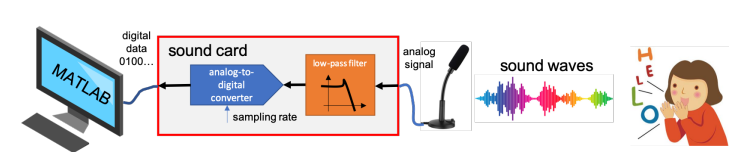
\includegraphics[scale=0.70]{Chapter3/blockDiagram}
\caption{Simplified block diagram of a microphone, sound-card, and computer. The microphone converts
air pressure into voltages, which are filtered and sampled. The samples are then transferred to MATLAB.}
\label{blockDiagram}
\end{center}
\end{figure}

\section{Flow Diagram}
Figure \ref{flowDiagram} shows the flow of the decimate function. In this project decimate function is the main function which we are using to process our signal with different factors.Decimation reduces the original sampling rate for a sequence to a lower rate, the opposite of interpolation. The decimation process filters the input data with a low pass filter and then resamples the resulting smoothed signal at a lower rate.\\\\
y = decimate(x,r) reduces the sample rate of x, the input signal, by a factor of r. The decimated vector, y, is shortened by a factor of r so that \\
\begin{center}
$length(y) = ceil(length\frac{x}{r})$
\end{center}
By default, decimate uses a low pass Chebyshev Type I infinite impulse response (IIR) filter of order 8.
\begin{figure}[H]  %h=positioning
\begin{center}
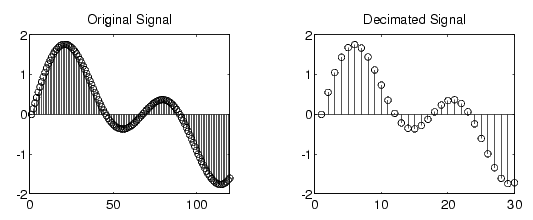
\includegraphics[scale=0.95]{Chapter3/DecimateASignalExample2}
\caption{Example of Decimating A Signal }
\label{DecimateASignalExample}
\end{center}
\end{figure}

\begin{figure}[H]  %h=positioning
\begin{center}
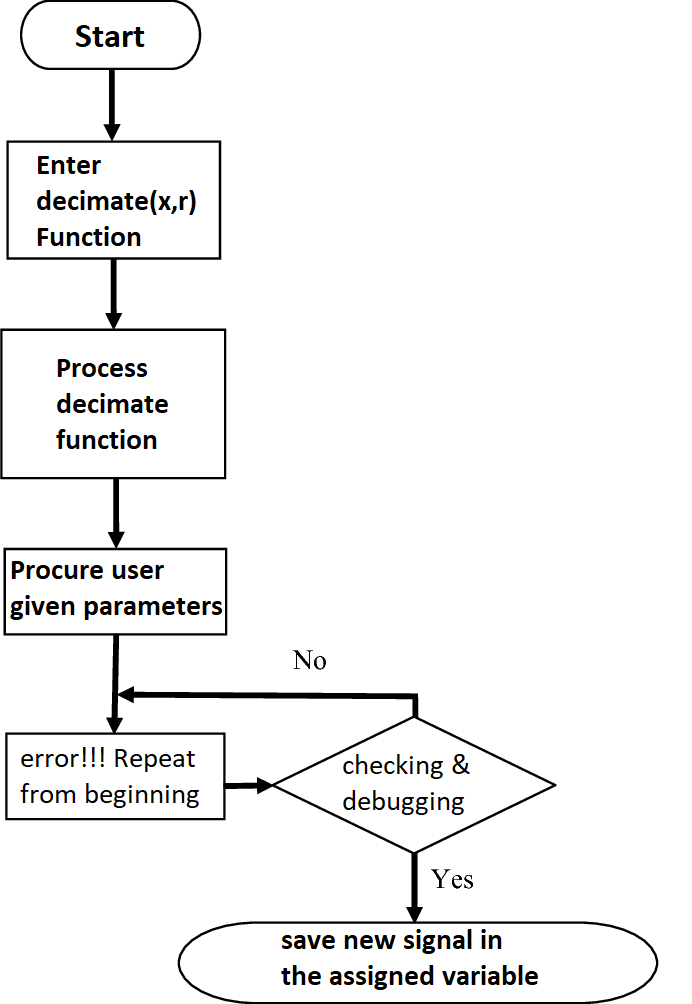
\includegraphics[scale=0.60]{Chapter3/flowDiagram}
\caption{Flow Diagram of the Project}
\label{flowDiagram}
\end{center}
\end{figure}

\section{System Model}
DSP System Toolbox provides algorithms and tools for the design and simulation of signal processing systems. These capabilities are provided as MATLAB functions, MATLAB System objects, and Simulink blocks. The system toolbox includes design methods for specialized FIR and IIR filters, FFTs, multirate processing, and DSP techniques for processing streaming data and creating real-time prototypes.\\\\
You can design adaptive and multirate filters, implement filters using computationally efficient architectures, and simulate floating-point digital filters. Tools for signal I/O from files and devices, signal generation, spectral analysis, and interactive visualization enable you to analyze system behavior and performance. For rapid prototyping and embedded system design, the system toolbox supports fixed-point arithmetic and C or HDL code generation.

\begin{figure}[H]  %h=positioning
\begin{center}
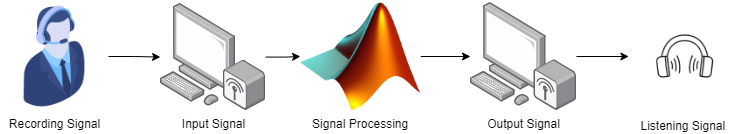
\includegraphics[scale=0.60]{Chapter3/systemModel}
\caption{System Model of the Project}
\label{systemModel}
\end{center}
\end{figure}


\section{Component Selection}
Signal processing engineers use MATLAB and Simulink at all stages of development�from analyzing signals and exploring algorithms to evaluating design implementation tradeoffs for building real-time signal processing systems. MATLAB and Simulink offer:
\begin{enumerate}
\item Built-in functions and apps for analysis and preprocessing of time-series data, spectral and time-frequency analysis, and signal measurements
%
\item Apps and algorithms to design, analyze, and implement digital filters (FIR and IIR) from basic FIR and IIR filters to adaptive, multirate, and multistage designs
%
\item An environment to model and simulate signal processing systems with a combination of programs and block diagrams
%
\item Capabilities to model fixed-point behavior and automatically generate C/C++ or HDL code for deploying on embedded processors, FPGAs, and ASICs
%
\item Tools for developing predictive models on signals and sensor data using machine learning and deep learning workflows
%
\end{enumerate}

{ \small \bfseries Note: Make sure you are using MATLAB 2013 or any less Version because wavrecord, wavplay are being replaced with audiorecorder/getaudiodata.}
\begin{figure}[H]  %h=positioning
\begin{center}
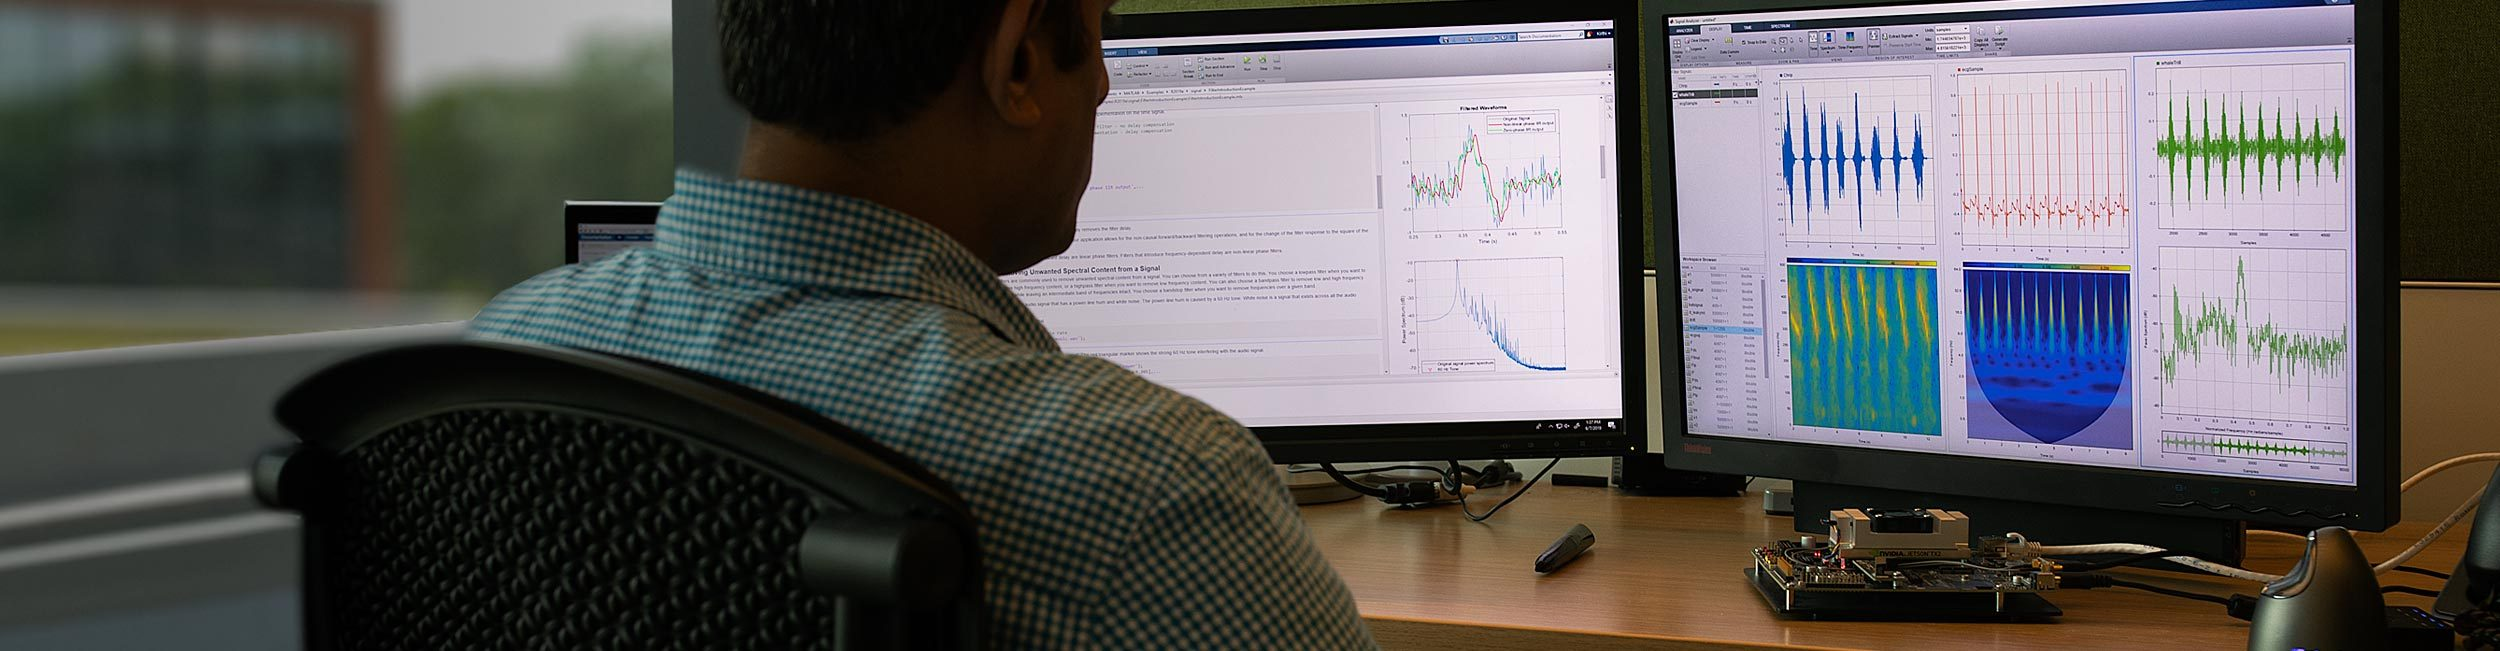
\includegraphics[scale=0.18]{Chapter3/aPersonUsingMATLAB}
\caption{Signal processing engineer using MATLAB and Simulink}
\label{aPersonUsingMATLAB}
\end{center}
\end{figure}

\chapter{Simulation and Results}
\label{chap4}
In the previous chapter, we have discussed about our methodology for this project while giving details about block diagram, system model, flow chart, software selection of this project. In this chapter, we will provide source code, and simulation and results of the project.
\section{Simulation Results}
As discussed in the previous chapter in the section of software selection, we have used MATLAB to simulate our project.
We have used two MATLAB function. In the first file, we have used that for the recording of the input signal where as the second file is accessing the input signal while calling that audio signal file and is performing the rest of the operation on that. Each line is properly comment to understand the use of that command.\\
{ \small \bfseries Note: Make sure both file should be in the same folder.}
\section{Source Code}
  \begin{lstlisting}[frame=single]
    % First(1) File
clc %Clear command window.
close all %closes all the open figure windows.

% sampling frequency
F = 32000;

%  recording speech on MATLAB
%  5*F is recording speech of 5 secs of sampling frequency
%  datatype to store the sound

y  = wavrecord(5*F, F, 'int16');
%Record sound using Windows audio input device.
%Y = wavrecord(N,FS,CH) records N audio samples at FS Hertz from
%CH number of input channels from the Windows WAVE audio device.
%playing recorded speech

wavplay(y, F);
% wavplay Play sound using Windows audio output device.
%wavplay(Y,FS) sends the signal in vector Y with sample frequency
%of FS Hertz to the Windows WAVE audio device.

audiowrite('project.wav',y, F)
%it will write the speech signal of the current file(save in memory)
%audiowrite write audio files
%audiowrite(FILENAME,Y,FS)  writes data Y to an audio
%file specified by the file name FILENAME, with a sample rate
%of FS Hz.
  \end{lstlisting}
  
\begin{lstlisting}[frame=single]
    % Second(2) File
clc
% (part a)
% wavread will read the .wav file in which speech is recorded
% y is samples or the input signal
% fs is the sampling frequency
[y,fs] = wavread('project.wav');
wavplay(y,fs);   %wavplay Play sound using Windows audio output device.
subplot(2,1,1)
% plotting frequency spectrum
% y is input signal
%freqz Frequency response of digital filter
freqz(abs(y))
% setting axis limits
x = linspace(0,0.1);    %linspace Linearly spaced vector.
xlim([0 0.1])   % xlim X limits.
ylim([-80 80])  % ylim Y limits.
title('Freq doamin magnitude spectrum of speech.');
subplot(2,1,2)% subplot Create axes in tiled positions.
% plotting time spectrum
plot(y),grid on;            % Linear plot &  Grid lines.
title('Time domain');       %Graph title.
xlabel('Seconds');         %X-axis label.
ylabel('Apmlitude');        %ylabel

% figure used to make the graphs appear in different windows
figure;
% fft is Fourier Transform to find highest frequency of signal
z=fft(y);
plot(abs(z)),grid on;           % Linear plot &  Grid lines.
title('Highest frequency');     %graph title
xlabel('Freq Hz');              %x-axis label
ylabel('Power');                %y-axis label

figure;
% (part b)
subplot(2,1,1)% subplot Create axes in tiled positions.
% decimating or downsampling the speech by facor 2
y1 = decimate(y,2)
%decimate is a low pass filter
freqz(abs(y1))%freqz frequency response of digital filter
x = linspace(0,0.1);    %linspace Linearly spaced vector.
xlim([0 0.1])           %x-axis limit
ylim([-80 80])          %y-axis limit
title('Freq doamin magnitude spectrum after decimating by 2');%graph title
subplot(2,1,2)% subplot Create axes in tiled positions.
plot(y1),grid on;% Linear plot &  Grid lines.
title('Time domain');       %graph title
xlabel('Seconds');          %x-axis label
ylabel('Apmlitude');        %y-axis label
wavplay(y1,fs);   %wavplay Play sound using Windows audio output device.


figure;         % figure Create figure window.
% (part c)
subplot(2,1,1)
% decimating by 4
y2 = decimate(y,2*2)
%decimate Resample data at a lower rate after lowpass filtering.
freqz(abs(y2))%freqz frequency response of digital filter.
x = linspace(0,0.1); %linearly spaced vector.
xlim([0 0.1]) %x-axis limit
ylim([-80 80])%y-axis limit
title('Freq Doamin Magnitude Spectrum After Decimating by 4');%graph title
subplot(2,1,2)% subplot Create axes in tiled positions.
plot(y2),grid on;% Linear plot &  Grid lines.
title('Time domain'); %graph title
xlabel('Seconds'); %x-axis label
ylabel('Apmlitude');%y-axis label
wavplay(y2,fs); %wavplay play sound using windows audio output device.


figure; %create figure window
% (part d)
subplot(2,1,1)% subplot Create axes in tiled positions.
% decimating by 8
y3 = decimate(y,2*2*2)
%decimate resample data at a lower rate after lowpass filtering
freqz(abs(y3)) %frequency response of digital filter.
x = linspace(0,0.1); %linearly spaced vector
xlim([0 0.1]) %x-axis limit
ylim([-60 60])%y-axis limit
title('Freq doamin magnitude spectrum after decimating by 8');%graph title
subplot(2,1,2)% subplot Create axes in tiled positions.
plot(y3),grid on;% Linear plot &  Grid lines.
title('Time domain'); %graph title
xlabel('Seconds');%x-axis label
ylabel('Apmlitude');%y-axis label
wavplay(y3,fs); %plays sound using windows audio output device


figure;%create figure window
% (part e)
subplot(2,1,1)% subplot Create axes in tiled positions.
% decimating by 16
% decimate resample data at a lower rate after lowpass filtering
y4 = decimate(y,2*2*2*2)
freqz(abs(y4))%frequency response of digital filter.
x = linspace(0,0.1);%linearly spaced vector
xlim([0 0.1])%x-axis limit
ylim([-50 50])%y-axis limit
title('Freq doamin magnitude spectrum after decimating by 16');%graph title
subplot(2,1,2)% subplot Create axes in tiled positions.
plot(y4),grid on;% Linear plot &  Grid lines.
title('Time domain');%graph title
xlabel('Seconds');%x-axis label
ylabel('Apmlitude');%y-axis label
wavplay(y4,fs);%plays sound using windows audio output device

z=fft(y4);
figure;
plot(abs(z)),grid on;
\end{lstlisting}
\clearpage
\section{Statistical Analysis}
\label{analysis}
Frequency spectrum of Input signal and  input signal in time domain is Fig. \ref{result1} .
\begin{figure}[H]  %h=positioning
\begin{center}
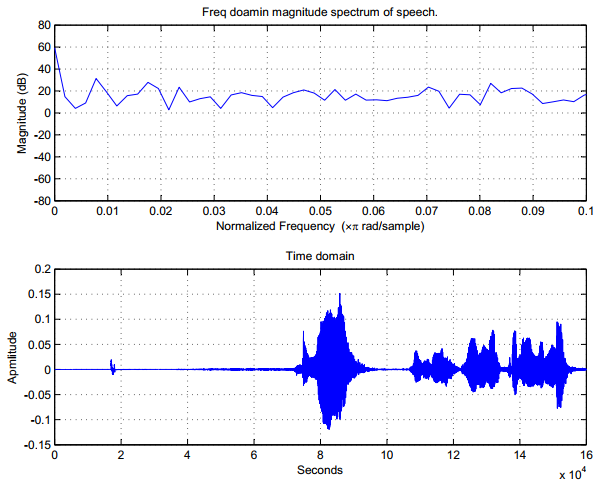
\includegraphics[scale=0.80]{Chapter4/result1}
\caption{Comparison of Frequency Spectrum and Time Domain Graph of Input Signal }
\label{result1}
\end{center}
\end{figure}

The highest frequency of recorded speech signal is 327kHz from fft is Fourier Transform to find highest frequency of signal which is shown in Fig. \ref{result2}

\begin{figure}[H]  %h=positioning
\begin{center}
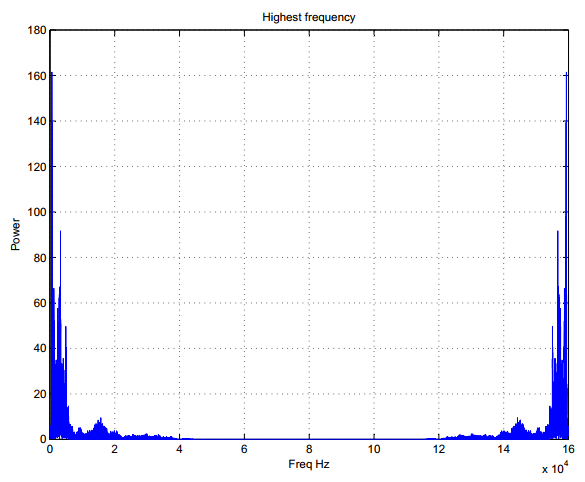
\includegraphics[scale=0.65]{Chapter4/result2}
\caption{Fourier Transform of the Input Signal }
\label{result2}
\end{center}
\end{figure}
Data transmitted per unit time is increased so does the speed of transmission or the speed
of speech is increased. Another thing we observed by decimating by 2 is that the
amplitude of frequency magnitude spectrum is got lowered from amplitude of original
frequency magnitude spectrum.\\\\
 
For example, if we take any sample point let�s say at 0.1,
the amplitude of original frequency magnitude spectrum at that sample point is almost
30dB but when decimated by 2 the amplitude of decimated frequency magnitude
spectrum goes to 28dB. Therefore, speech is not that much clear to understand than
original speech and time is reduced as shown in the Fig. \ref{result3}.

\begin{figure}[H]  %h=positioning
\begin{center}
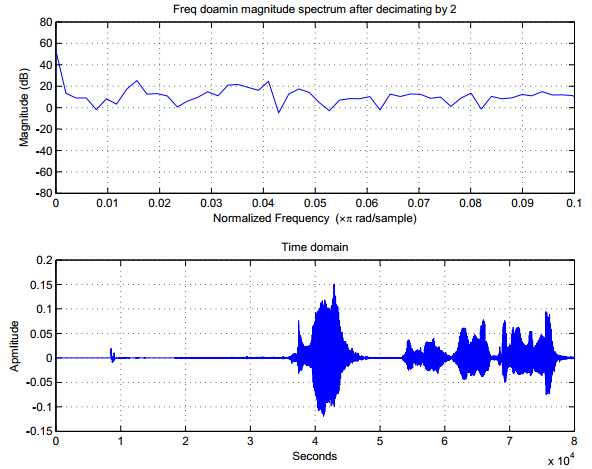
\includegraphics[scale=0.90]{Chapter4/result3}
\caption{Comparison of Frequency Spectrum and Time Domain Graph of Input Signal After Decimating by 2 }
\label{result3}
\end{center}
\end{figure}
Data transmitted rate is much more increased. By decimating by 4 the amplitude of
frequency magnitude spectrum is got much lowered from amplitude of original frequency
magnitude spectrum.\\\\
 For example, if we take any sample point let�s say at 0.1, the amplitude of original frequency magnitude spectrum at that sample point is almost 30dB but when decimated by 4 the amplitude of decimated frequency magnitude spectrum goes
to 25dB. The decimated speech is very rough and not clear enough to understand because
time is more decreased as shown in the Fig. \ref{result4}.

\begin{figure}[H]  %h=positioning
\begin{center}
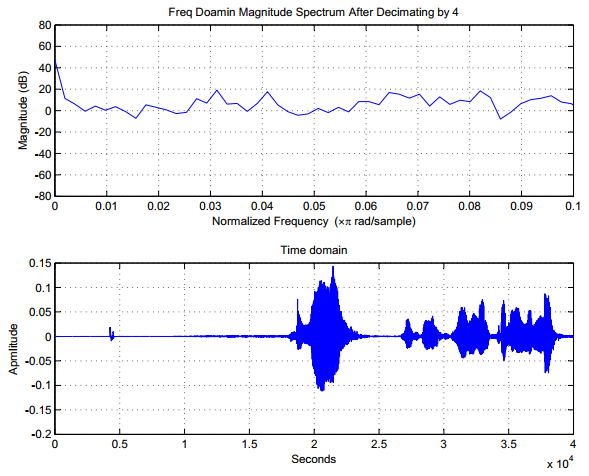
\includegraphics[scale=0.90]{Chapter4/result4}
\caption{Comparison of Frequency Spectrum and Time Domain Graph of Input Signal After Decimating by 4 }
\label{result4}
\end{center}
\end{figure}


Decimation reduces the original sample rate of a sequence to a lower rate. It is the opposite of interpolation. decimate lowpass filters the input to guard against aliasing and downsamples the result. When using the FIR filter, decimate filters the input sequence in only one direction. This conserves memory and is useful for working with long sequences. In the IIR case, decimate applies the filter in the forward and reverse directions using filtfilt to remove phase distortion. In effect, this process doubles the filter order. In both cases, the function minimizes transient effects at both ends of the signal by matching endpoint conditions\\\\
Data transmitted per unit time is much more increased and the speed of transmission or
the speed of speech is increased. Another thing we observed by decimating by 8 is that
the amplitude of frequency magnitude spectrum is got lowered from amplitude of original
frequency magnitude spectrum.\\\\
For example, if we take any sample point lets say at 0.1,
the amplitude of original frequency magnitude spectrum at that sample point is almost
30dB but when decimated by 8 the amplitude of decimated frequency magnitude
spectrum goes to 18dB. The speech is played so fast that the speech is almost impossible
to understand, time is much more reduced as shown in the Fig.\ref{result5}.

\begin{figure}[H]  %h=positioning
\begin{center}
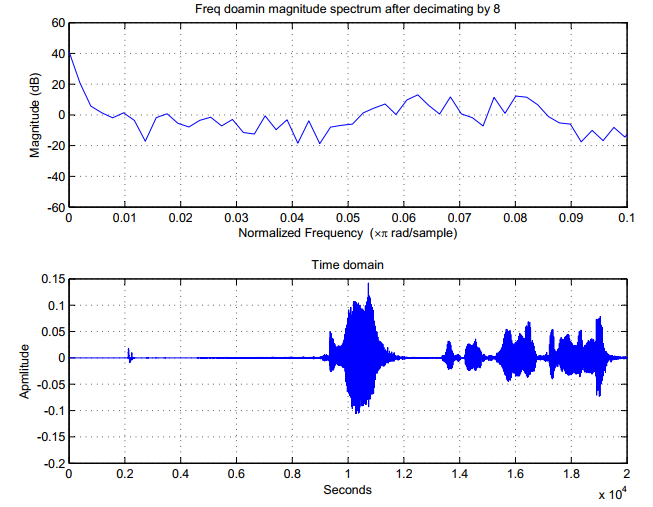
\includegraphics[scale=0.90]{Chapter4/result5}
\caption{Comparison of Frequency Spectrum and Time Domain Graph of Input Signal After Decimating by 8}
\label{result5}
\end{center}
\end{figure}

decimate creates a lowpass filter. The default is a Chebyshev Type I filter designed using cheby1. This filter has a normalized cutoff frequency of 0.8/r and a passband ripple of 0.05 dB. Sometimes, the specified filter order produces passband distortion due to round-off errors accumulated from the convolutions needed to create the transfer function. decimate automatically reduces the filter order when distortion causes the magnitude response at the cutoff frequency to differ from the ripple by more than $1/10^6$.\\
When the 'fir' option is chosen, decimate uses fir1 to design a lowpass FIR filter with cutoff frequency $1/r$.\\\\
Data transmitted per unit time is so much increased Another thing we observed by
decimating by 16 is that the amplitude of frequency magnitude spectrum is got lowered
from amplitude of original frequency magnitude spectrum.\\\\
For example, if we take any sample point let�s say at 0.1, the amplitude of original frequency magnitude spectrum at
that sample point is almost 30dB but when decimated by 16 the amplitude of decimated
frequency magnitude spectrum almost goes to 1dB. The rate of speech is so less that the
speech is impossible to understand, time is much more reduced as shown in the Fig. \ref{result6}.

\begin{figure}[H]  %h=positioning
\begin{center}
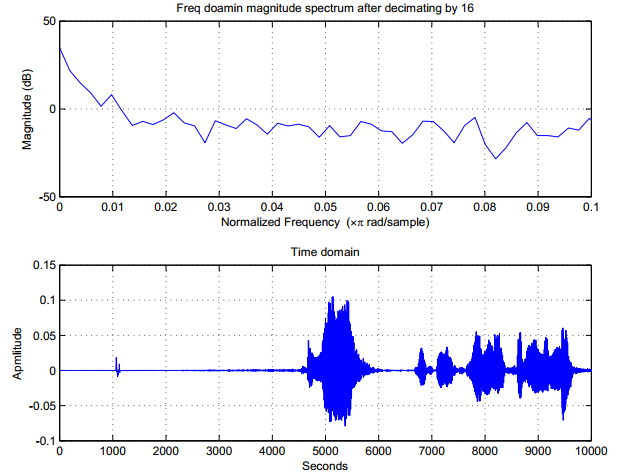
\includegraphics[scale=0.90]{Chapter4/result6}
\caption{Comparison of Frequency Spectrum and Time Domain Graph of Input Signal After Decimating by 16}
\label{result6}
\end{center}
\end{figure}
\chapter{Conclusion and Future Work}
\label{chap5}
In the previous chapter, we have shown all the simulation and results of our proposed project. From introduction, Literature Review, Proposed Methodology, Result and Simulations. In this chapter, we will conclude our project and will 
\section{Conclusion}
This work describes the speech processing using MATLAB. We have:
\begin{enumerate}
\item Describe signals mathematically and understand
how to perform mathematical operations on signals.
%
\item This project provides knowledge of Digital filter
%
\item discuss word length issues ,multi rate signal processing and application
%
\end{enumerate}
In this project, we have record our speech of about 5 seconds at sampling frequency of 32 kHz.
we have use either �wavrecord()� MATLAB function\\
After that we have:
\begin{enumerate}
\item Plotted the time and frequency domain magnitude spectrums of this speech signal.
 And found 327kHz is highest frequency of this signal and played that signal using
�wavplay()�.
%
\item We have decimated the signal by a factor of 2 repeatedly. And again plotted the time and frequency domain
spectrum of the signal. And played the sound. Observation of this step is mentioned in detail in the Chapter \ref{chap4}.

%
\end{enumerate}

\section{Future Work}
Speech processing using MATLAB can be done in many other ways and the current method/project can be improve in many ways. Following are the some of the things we can try to improve this system:
\begin{enumerate}
\item Different method of the signal processing can be used to improve it.
%
\item High quality microphone can be used to improve the system accuracy.
%
%
\item Instead of using wavrecord, wavplay we can create the same project with the updated commands like audiorecorder/getaudiodata in MATLAB.
%
\item We can try on implementing the processing technique on multi subjects.
\end{enumerate}

%\include{Chapter6/Chapter6}
%\include{Chapter8/Chapter8}
%\include{Chapter7/Chapter7}

\bibliographystyle{ieeetr}
\bibliography{Ref}
\end{document}
